\documentclass[]{elsarticle} %review=doublespace preprint=single 5p=2 column
%%% Begin My package additions %%%%%%%%%%%%%%%%%%%
\usepackage[hyphens]{url}

  \journal{IPEA Working Papers} % Sets Journal name


\usepackage{lineno} % add
\providecommand{\tightlist}{%
  \setlength{\itemsep}{0pt}\setlength{\parskip}{0pt}}

\usepackage{graphicx}
\usepackage{booktabs} % book-quality tables
%%%%%%%%%%%%%%%% end my additions to header

\usepackage[T1]{fontenc}
\usepackage{lmodern}
\usepackage{amssymb,amsmath}
\usepackage{ifxetex,ifluatex}
\usepackage{fixltx2e} % provides \textsubscript
% use upquote if available, for straight quotes in verbatim environments
\IfFileExists{upquote.sty}{\usepackage{upquote}}{}
\ifnum 0\ifxetex 1\fi\ifluatex 1\fi=0 % if pdftex
  \usepackage[utf8]{inputenc}
\else % if luatex or xelatex
  \usepackage{fontspec}
  \ifxetex
    \usepackage{xltxtra,xunicode}
  \fi
  \defaultfontfeatures{Mapping=tex-text,Scale=MatchLowercase}
  \newcommand{\euro}{€}
\fi
% use microtype if available
\IfFileExists{microtype.sty}{\usepackage{microtype}}{}
\bibliographystyle{elsarticle-harv}
\usepackage{color}
\usepackage{fancyvrb}
\newcommand{\VerbBar}{|}
\newcommand{\VERB}{\Verb[commandchars=\\\{\}]}
\DefineVerbatimEnvironment{Highlighting}{Verbatim}{commandchars=\\\{\}}
% Add ',fontsize=\small' for more characters per line
\usepackage{framed}
\definecolor{shadecolor}{RGB}{248,248,248}
\newenvironment{Shaded}{\begin{snugshade}}{\end{snugshade}}
\newcommand{\AlertTok}[1]{\textcolor[rgb]{0.94,0.16,0.16}{#1}}
\newcommand{\AnnotationTok}[1]{\textcolor[rgb]{0.56,0.35,0.01}{\textbf{\textit{#1}}}}
\newcommand{\AttributeTok}[1]{\textcolor[rgb]{0.77,0.63,0.00}{#1}}
\newcommand{\BaseNTok}[1]{\textcolor[rgb]{0.00,0.00,0.81}{#1}}
\newcommand{\BuiltInTok}[1]{#1}
\newcommand{\CharTok}[1]{\textcolor[rgb]{0.31,0.60,0.02}{#1}}
\newcommand{\CommentTok}[1]{\textcolor[rgb]{0.56,0.35,0.01}{\textit{#1}}}
\newcommand{\CommentVarTok}[1]{\textcolor[rgb]{0.56,0.35,0.01}{\textbf{\textit{#1}}}}
\newcommand{\ConstantTok}[1]{\textcolor[rgb]{0.00,0.00,0.00}{#1}}
\newcommand{\ControlFlowTok}[1]{\textcolor[rgb]{0.13,0.29,0.53}{\textbf{#1}}}
\newcommand{\DataTypeTok}[1]{\textcolor[rgb]{0.13,0.29,0.53}{#1}}
\newcommand{\DecValTok}[1]{\textcolor[rgb]{0.00,0.00,0.81}{#1}}
\newcommand{\DocumentationTok}[1]{\textcolor[rgb]{0.56,0.35,0.01}{\textbf{\textit{#1}}}}
\newcommand{\ErrorTok}[1]{\textcolor[rgb]{0.64,0.00,0.00}{\textbf{#1}}}
\newcommand{\ExtensionTok}[1]{#1}
\newcommand{\FloatTok}[1]{\textcolor[rgb]{0.00,0.00,0.81}{#1}}
\newcommand{\FunctionTok}[1]{\textcolor[rgb]{0.00,0.00,0.00}{#1}}
\newcommand{\ImportTok}[1]{#1}
\newcommand{\InformationTok}[1]{\textcolor[rgb]{0.56,0.35,0.01}{\textbf{\textit{#1}}}}
\newcommand{\KeywordTok}[1]{\textcolor[rgb]{0.13,0.29,0.53}{\textbf{#1}}}
\newcommand{\NormalTok}[1]{#1}
\newcommand{\OperatorTok}[1]{\textcolor[rgb]{0.81,0.36,0.00}{\textbf{#1}}}
\newcommand{\OtherTok}[1]{\textcolor[rgb]{0.56,0.35,0.01}{#1}}
\newcommand{\PreprocessorTok}[1]{\textcolor[rgb]{0.56,0.35,0.01}{\textit{#1}}}
\newcommand{\RegionMarkerTok}[1]{#1}
\newcommand{\SpecialCharTok}[1]{\textcolor[rgb]{0.00,0.00,0.00}{#1}}
\newcommand{\SpecialStringTok}[1]{\textcolor[rgb]{0.31,0.60,0.02}{#1}}
\newcommand{\StringTok}[1]{\textcolor[rgb]{0.31,0.60,0.02}{#1}}
\newcommand{\VariableTok}[1]{\textcolor[rgb]{0.00,0.00,0.00}{#1}}
\newcommand{\VerbatimStringTok}[1]{\textcolor[rgb]{0.31,0.60,0.02}{#1}}
\newcommand{\WarningTok}[1]{\textcolor[rgb]{0.56,0.35,0.01}{\textbf{\textit{#1}}}}
\usepackage{graphicx}
% We will generate all images so they have a width \maxwidth. This means
% that they will get their normal width if they fit onto the page, but
% are scaled down if they would overflow the margins.
\makeatletter
\def\maxwidth{\ifdim\Gin@nat@width>\linewidth\linewidth
\else\Gin@nat@width\fi}
\makeatother
\let\Oldincludegraphics\includegraphics
\renewcommand{\includegraphics}[1]{\Oldincludegraphics[width=\maxwidth]{#1}}
\ifxetex
  \usepackage[setpagesize=false, % page size defined by xetex
              unicode=false, % unicode breaks when used with xetex
              xetex]{hyperref}
\else
  \usepackage[unicode=true]{hyperref}
\fi
\hypersetup{breaklinks=true,
            bookmarks=true,
            pdfauthor={},
            pdftitle={Estimating the value of travel time saving and statistical life in road travels in Brazil (English Short version)},
            colorlinks=false,
            urlcolor=blue,
            linkcolor=magenta,
            pdfborder={0 0 0}}
\urlstyle{same}  % don't use monospace font for urls

\setcounter{secnumdepth}{5}
% Pandoc toggle for numbering sections (defaults to be off)
% Pandoc header
\usepackage{booktabs}
\usepackage{longtable}
\usepackage{array}
\usepackage{multirow}
\usepackage{wrapfig}
\usepackage{float}
\usepackage{colortbl}
\usepackage{pdflscape}
\usepackage{tabu}
\usepackage{threeparttable}
\usepackage{threeparttablex}
\usepackage[normalem]{ulem}
\usepackage{makecell}
\usepackage{xcolor}



\begin{document}
\begin{frontmatter}

  \title{Estimating the value of travel time saving and statistical life in road
travels in Brazil (English Short version)}
    \author[IPEA - Institute of Applied Economic Research (DISET)]{Tatiana Ferrari\corref{c1}}
   \ead{tatianak.ferrari@gmail.com} 
   \cortext[c1]{Corresponding Author}
    \author[IPEA - Institute of Applied Economic Research (DISET)]{Luisa Dusi}
   \ead{luiza.dusi@ipea.gov.br} 
  
    \author[IPEA - Institute of Applied Economic Research (DISET)]{Fabiano Pompemayer}
   \ead{fabiano.pompermayer@ipea.gov.br} 
  
      \address[IPEA - Institute of Applied Economic Research (DISET)]{IPEA - Institute of Applied Economic Research. Setor Bancario Sul,
Quadra 1, Edificio BNDES, Brasilia, DF, Brazil}
  
  \begin{abstract}
  In this paper, we discuss the methodological procedures and the
  computation of the value of travel time saving and value of statistical
  life in road travels in Brazil. A stated preference experiment was
  carried out, in which we bring some innovations in order to control for
  hypothetical bias. The survey was conducted online through the snowball
  technique, requesting respondents to choose between two hypothetical
  routes with different levels of three attributes: toll cost, time and
  number of deaths. The mixed logit model was used to estimate the
  willingness to pay for the travel time saving and for the death risk
  reduction. The results show significant difference in the values given
  the certainty level in the individual´s answer. The model is also
  estimated controlled for travel and individual characteristics. Despite
  the important results found, the first ones in our knowledge for the
  Brazilian context, the data collection was biased which made it
  impossible to extrapolate the results to the population.
  \end{abstract}
  
 \end{frontmatter}

\hypertarget{introduction}{%
\section{Introduction}\label{introduction}}

Brazil has a road network of about 1.8 million kilometers, being the
main means of transportation in the country. However, data from the
Highway Survey conducted by the National Transport Confederation (CNT,
2016) show that the general state of Brazilian roads is deficient: only
12.3\% of the roads are paved, 86.6\% are single carriageways and 42.2\%
have no shoulder. According to the evaluation carried out by CNT,
deficiencies in roads cause high fuel consumption, greater wear and tear
on the vehicle fleet, greater occurrence of accidents and environmental
damage. In addition, roads with limited capacity and boreholes
considerably increase travel time.

Pompermayer (2017) shows that the average annual expenditures of the
National Department of Transportation Infrastructure (DNIT), only with
recovery and maintenance of the Brazilian road network, are more than
R\$ 8 billion and still insufficient to maintain an acceptable quality
standard.

The scarce resources cause public policy makers to prioritize different
investments in road infrastructure. Improvements in the condition of
roads can result in important gains in reducing travel time, reducing
vehicle costs and maintenance, and reducing the number of fatal
accidents. Thus, intervention projects can be justified through
cost-benefit analyses. For this, it is necessary to obtain the monetary
values of such benefits.

According to the microeconomic theory of revealed preference, the value
of goods and services can be derived by observing the choices made by
individuals. However, time and the reduction of the risk of death do not
have market value, because they are not tangible and subjective
benefits.

In view of this, the study aims to obtain estimates related to the
parameters of time savings value and the value of statistical life for
the Brazilian case, in order to subsidize cost-benefit analyses of
investment projects in highways, as well as in other projects or
policies involving these parameters. The methodology used consisted of
survey application to obtain the declared preference (PD) of individuals
and the use of the Mixed Multinomial Logit model, of discrete choice, to
estimate the willingness to pay (WTP) for these attributes.

The rest of this paper is organized as follows. Section 2 describes
briefly the topics in the survey; Section 3 the methodology adopted for
preference analysis; and Section 4 presents the estimation results.

\hypertarget{survey-design}{%
\section{Survey Design}\label{survey-design}}

\hypertarget{survey-structure}{%
\subsection{Survey Structure}\label{survey-structure}}

The survey consists of seven sections, namely:

\begin{enumerate}
\def\labelenumi{(\arabic{enumi})}
\item
  Introduction and first set of social-economic data;
\item
  Travel habits from last 12 months;
\item
  Last or most frequent trip made by car or motorcycle in Brazilian
  highways;
\item
  Stated choice experiment;
\item
  Debrief;
\item
  Complementary questions;
\item
  Second set of social-economic data.
\end{enumerate}

One question in particular is worth pointing out: we asked the
respondents about their involvement in accidents, or of their relatives.
To test if the recollection of a possible/actual accident would
influence their choice behavior when answering the experiment we
randomized the position of this question: either immediately before or
after the experiment.

\hypertarget{methodology}{%
\section{Methodology}\label{methodology}}

Estimates for the value of travel time savings and of risk of death
reduction on roads travels was obtained by applying the discrete choice
model. This approach considers that each individual \emph{n} has a set
of alternatives, each having a series of associated characteristics
(\(x_{nj}\)). The individual will choose the alternative that maximizes
their utility, account for observable and unobserved factors, so that
\(U_{ni} > U_{nj}\) for \(\forall j\neq i\).:

\[
U_{nj} = V_{ni} + \epsilon_{ni} = \beta^{'}_{n} X_{nj} + \epsilon_{nj}
\]

where \(x_{nj}\) is a vector of observed variables that gives the
utility of individual \emph{n} for the alternative \emph{i}, \(\beta_n\)
is the correspondent vector of coefficients of variables \(x_{nj}\)
representing the individual's tastes, and \(\epsilon_{ni}\) is an
unobserved random term that represents the effects of omitted variable.

The route choice process of our stated preference experiment allow us to
derive the subjective valuations of the attributes, which are called
Willingness to Pay (WTP) and expresses the marginal substitution rate
between the considered attribute and the cost, given a constant utility.

Among the different class of models, we find the the mixed logit model
more appropriate for modeling our choice data, since it allows the
coefficients of the model to have variations between the individuals.
According to Train (2002), the mixed logit probabilities are the
integral of standard logit probabilities over a density of parameters.
If the utility is linear in \(\beta\), can be expressed as:

\begin{equation}
    P_{ni} = \int \frac{exp(x'_{ni}\beta)}{\sum^J_{j=1}exp(x'_{nj}\beta)}f(\beta|\theta)d\beta
\label{eq:mixed_form}
\end{equation}

where, \(x'_{ni}\beta\) are the portion of utility observed, which
depends on parameters \(\beta\) and \(f(\beta|\theta)\) is a density
function of \(\beta\). In this terms, the mixed logit model is a mixture
of a logit function evaluated in different \(\beta\)'s, with a mixed
distribution in \(f(\beta|\theta)\).

In the stated preference experiment each respondent has a sequence of
route choice (nine times in our particular case). To count all of then
it is necessary to take the product of the Equation \ref{eq:mixed_form}:

\[
    S_{n} = \int \prod^T_{t=1} \prod^J_{j=1} \Bigg[\frac{exp(x'_{ni}\beta)}{\sum^J_{j=1}exp(x'_{nj}\beta)}\Bigg]^{y_{njt}}f(\beta|\theta)d\beta
\]

with, \(y_{njt}= 1\) if the alternative \emph{j} was choosen in
\emph{t}, and 0 otherwise.

As stated by Hensher and Greene (2003) the choice probability in mixed
logit models ``cannot be calculated exactly because the integral does
not have a closed form. The integral is approximated through
simulation''. The simulated probability (SP) that an individual chooses
alternative \emph{i} could be obtained through the maximization of the
likelihood function. In general, this simulation is given by a Halton's
sequence.

\begin{equation}
    SP = \sum^N_{n=1}ln \Big(\frac{1}{R} \sum^R_{r=1} \prod^T_{t=1} \prod^J_{j=1} \Bigg[\frac{exp(x'_{nit}\beta^{[r]}_n)}{\sum^J_{j=1}exp(x'_{njt}\beta^{[r]}_n)}\Bigg]^{y_{njt}} \Big)
\end{equation}

With \(\beta^{[r]}_n\) representing the number of drawings (r = number
of Halton's draws) for individual \emph{n} given the assumed
distribution by \(\beta\).

Thus, three specifications arise with the use of the mixed logit model:
1) select the variables that should be considered as random; 2) the
choice of the statistical distribution for the random coefficients; and
3) determine the number of Halton draws for the simulation.

The random variables included in the model are the ones of the stated
preference experiment: cost, time and risk of death. The other variables
that may be included, as the characteristics of the respondent and of
the travel, are treat as no random.

The normal distribution is the standard distribution in statistical
software and generally applied in mixed logit models. However, Hess et
al. (2005) shows that, since the normal distribution is unbounded, every
real number has a probability of being estimated in the simulation
process´´. In the case of parameters that have a strictly negative
distribution, but has a mean close to zero with a long tail into the
negative space of numbers´´, as in the case of time and risk of death
reduction, ``the symmetrical nature of the normal distribution can, in
approximation, lead to a significant share of positive values, even
though such values are not actually revealed by the data´´.

Hence, the following alternative distributions are tested: lognormal,
triangular and normal distribution truncated at zero. The better model
fit is obtained by the model using the Normal distribution truncated at
zero. In this case,

\begin{equation}
    \beta_{k,ir} = 
       \begin{cases}
            \beta_k + \omega_kW_{k.ir}, & \mbox{if } \beta_{k_ir} > 0 \\

             0, & \mbox{otherwise.} \\
       \end{cases} 
       W_{k_ir} ~ N(0,1)
\end{equation}

The third specification refers to the number of Halton draws to be
considered. The model were tested using different numbers of draws,
comparing the efficiency and time of processing. It was observed that
after 500 Halton draws the model stabilized, with no significant gains
in efficiency with the increase in number of simulations and therefore,
this number was established for the model.

\hypertarget{results}{%
\section{Results}\label{results}}

\hypertarget{general-model}{%
\subsection{General model}\label{general-model}}

We first approach a general model, considering only the game attributes:
cost, time and death.

Table \ref{resultgeral} presents the estimation of the respondent's
preferences according to the mixed logit model, considering the
specifications of section 3. The coefficients were significant at 1\%
and present the expected sign. It's important to emphasize that the
variable's signs were switched due to the truncated distribution adopted
previously. Therefore, the positive result for cost, time and death mean
an negative impact, that is, when traveling the individuals prefer the
route with lowest cost, travel time and death risk.

\begin{verbatim}
## 
## General Mixed Logit Result
## =====================================================
##                                choice                
## -----------------------------------------------------
## Intercept                -0.870*** (0.063)           
## Cost                      0.157*** (0.003)           
## Life                      0.359*** (0.009)           
## Time                      0.072*** (0.002)           
## sd.cost                   0.065*** (0.002)           
## sd.life                   0.324*** (0.012)           
## sd.time                   0.021*** (0.002)           
## N                              25,730                
## R2                             0.313                 
## Log Likelihood              -12,114.600              
## LR Test                11,032.590*** (df = 7)        
## =====================================================
## Notes:         ***Significant at the 1 percent level.
##                 **Significant at the 5 percent level.
##                 *Significant at the 10 percent level.
\end{verbatim}

\begin{table}[H]
\centering
\begin{tabular}{l|c|c}
\hline
  & WTP\_200km & Values\\
\hline
tempo & Time (BRL per hour) & 27.62\\
\hline
morte & Life(BRL per 1 death) & 2.29\\
\hline
\end{tabular}
\end{table}

Considering the baseline distance of 200km, the model estimated a
willingness to pay of R\$27,60 for a travel time saving of one hour and
R\$2,29 for risk reduction of one death.

The WTP values are random variables with an unknown distribution. With
the means and the standard deviation values of the variables, we used a
simulation process to estimate the values' distribution for individuals,
considering the interval of 0 to 100 Brazilian Reais.

Figure\ref{figure2} presents the distribution for WTP as a Kernel
Density. It is concentrated at the beginning of the distribution, where
values for WTP are lower. For death risk reduction, 95\% of the
distribution is concentrated up to BRL 10, while the WTP for travel time
saving seems to be more distributed and with a lengthened tail. However,
that occurs only due to the value conversion to value per hour.
Therefore, we have a strong concentration of individuals who are willing
to pay between BRL 10 and BRL 40 for the reduction of one hour in their
travel time.

\begin{Shaded}
\begin{Highlighting}[]
\NormalTok{fig1 <-}\StringTok{ }\KeywordTok{plot}\NormalTok{(}\KeywordTok{density}\NormalTok{( razao1[razao1 }\OperatorTok{<}\StringTok{ }\DecValTok{100}\NormalTok{] ), }\DataTypeTok{col =} \StringTok{"red"}\NormalTok{)}
\end{Highlighting}
\end{Shaded}

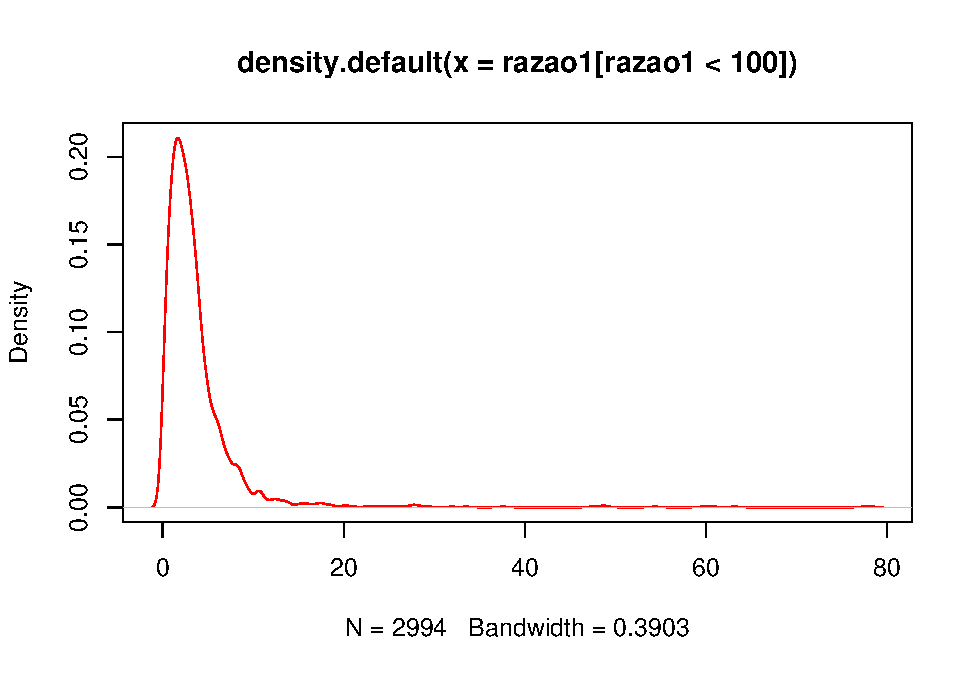
\includegraphics{WTP_transport_files/figure-latex/figure2-1.pdf}

\begin{Shaded}
\begin{Highlighting}[]
\CommentTok{# Recreate Figure 2}
\NormalTok{fig2 <-}\StringTok{ }\KeywordTok{plot}\NormalTok{(}\KeywordTok{density}\NormalTok{( razao2[razao2 }\OperatorTok{<}\StringTok{ }\DecValTok{100}\NormalTok{] ), }\DataTypeTok{col =} \StringTok{"blue"}\NormalTok{)}
\end{Highlighting}
\end{Shaded}

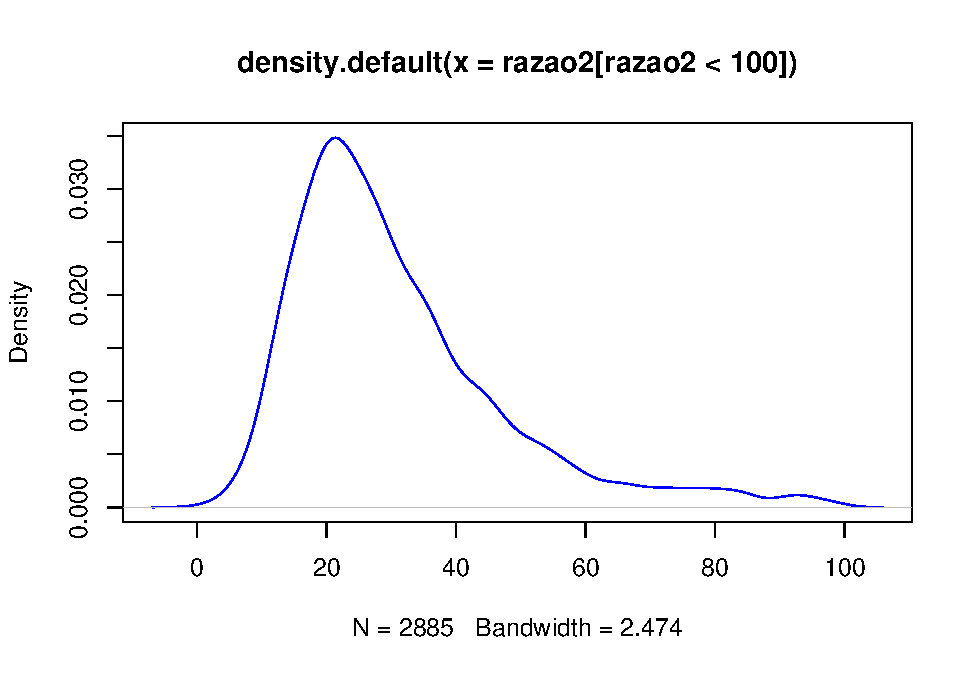
\includegraphics{WTP_transport_files/figure-latex/figure2-2.pdf}

\begin{Shaded}
\begin{Highlighting}[]
\CommentTok{# grid.arrange(fig1, fig2, ncol = 2)}
\end{Highlighting}
\end{Shaded}

One of the factors that can influence the individual's perception of the
value they're willing to pay is if they are - or are not - road users.
As stated by Sen (1993), information access can considerably change
individual's choice behaviour. Our survey informs respondents about
travel conditions as travel time and number of deaths by road accidents,
while also reminding them of their personal travel experience, as to
give context and therefore improve their perception when answering the
game. Nevertheless, we allowed all participants to respond to the game,
frequent travelers or not, who have travelled on roads in the last 12
months, as well as the ones who didn't.

As observed in Table \ref{table-simple}, there was a clear difference in
perception of users and non-users of roads. The ones who hadn't traveled
in the past 12 months had a WTP for reducing death risk significantly
higher than the ones who did travel, being willing to pay R\$0,90 more.

For travel time savings, it is interesting to notice that non-user
individuals had similar preferences, with the variable's standard
deviation being not significant, that is, the importance of time was
homogeneous between individuals of the stratum. The willingness to pay,
as with the previous parameter, was superior to the one of users.

This behaviour might be explained by difference in the amount of
knowledge and access to information that users and non-users have.
Non-users might have used their urban area commute experience as a
reference. Also, they don't have knowledge about other incurred travel
costs, road conditions and other aspects that might alter their
perception to the point of being willing to pay higher prices for
reduction of travel time and of death risk.

\begin{figure}
\centering
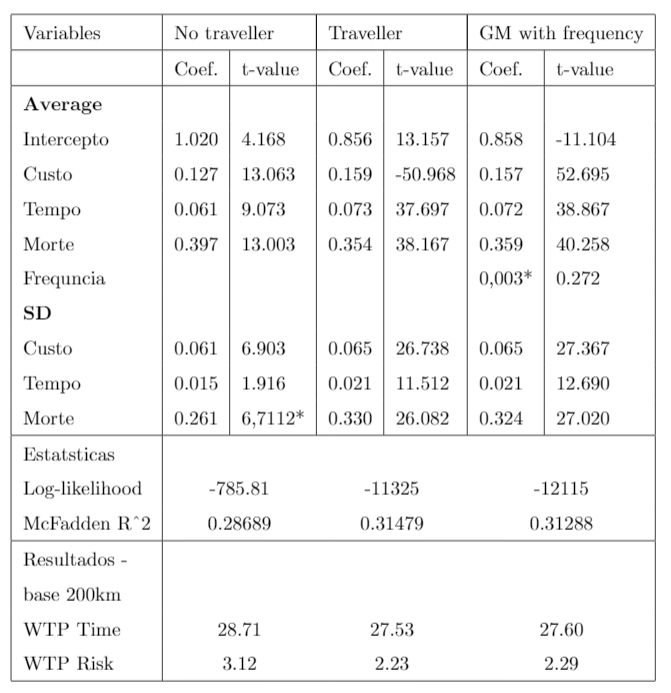
\includegraphics{table15.png}
\caption{Mixed Logit to travellers and no travellers.}
\end{figure}

Finally, in this general analysis, we estimated the WTP of respondents
according to the degree of certainty with which they answered the game.
The calibration through the certainty approach allows us to remove some
behavioural deviance inherent to the stated preference method. Since we
are applying a monetary value to an intangible good, that is, which
doesn't have a market value, the respondent might not be acquainted with
the object of choice and therefore have some difficulties when
evaluating their preferences for these goods.

The purpose of this approach is to exclude answers in which there was a
considerable amount of uncertainty declared. However, the literature
shows that there is no consensus regarding the acceptable degree of
certainty, as the review carried out by Beck et al. (2016) verified:
several studies use 8 and others use 7 as a threshold, amongst other
values.

Graphic 1 shows the pattern of answer certainty (CA) for each question
of the experiment. Most answers had a high level of certainty. Grades
from 7 to 10 summed over 80\% of answers in most questions. The ones
with a higher level of uncertainty, that is, more than 15\% of grades
under 7 (items: 3, 4, 13, 18, 19, 22, 23 and 27) are the ones with
highest value for toll (R\$40).

\begin{figure}
\centering
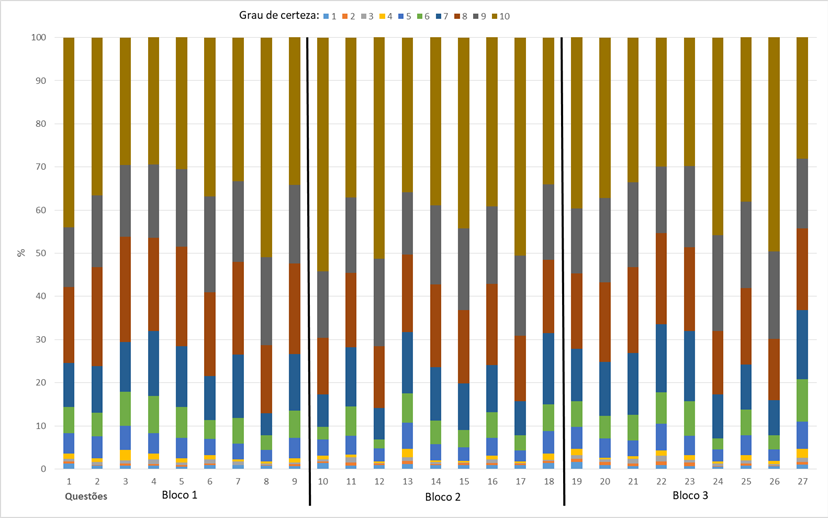
\includegraphics{CA.png}
\caption{Certainty approach report.}
\end{figure}

We separated the answers into three groups based on the declared degree
of certainty: Certain - CA from 7 to 10; Some certainty - CA from 4 to
6; Uncertain - CA up to 3.

The results of the mixed logit model estimation for each CA group is
presented on Table. Graphics and shows the Kernel Density for risk of
death reduction and travel time savings respectively.

We can observe that there is a significant variation in answer patterns
when considering the respondents certainty of choice. The results, in
addition, show that when the answer was made with uncertainty, the
estimations for the parameters of death, time and their respective
standard deviations weren't significant at 10\%. Notice that choices
made with certainty provided a higher value to death risk reduction and,
as the trade-off with cost became closer to the threshold (higher
prices), the level of certainty decreased.

This trade-off can easily be observed in the Kernel Density graphs
(Table and. The curve of uncertain answers is concentrated in lower
values of WTP while the certain answers is better distributed. In
contrast, the curve of uncertain choice also presents a distribution
with a tail with greater length. This pattern shows that the uncertainty
was generated in cases when the individual did not accept to pay a
higher price for improvement, but was not confident to renounce the
benefits, or that he agreed to pay the higher price for improvements but
disapproved the value proposed.

\begin{figure}
\centering
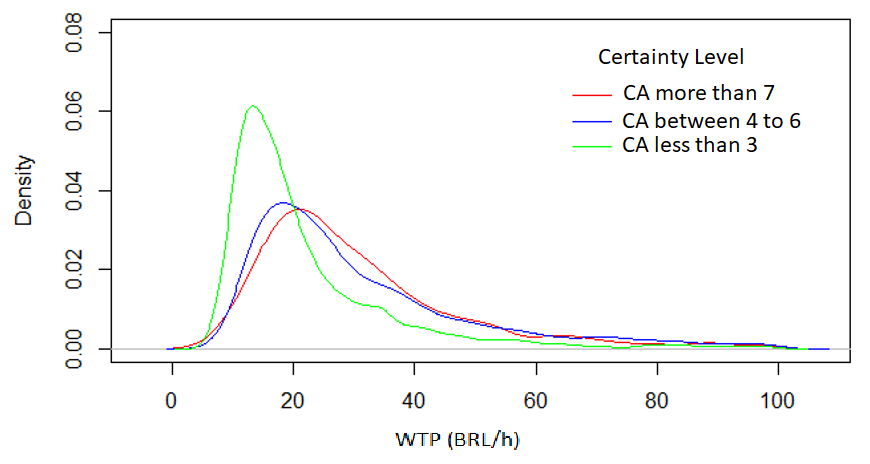
\includegraphics{dist_WTP_CAtime.png}
\caption{WTP distribution of travel time saving by CA.}
\end{figure}

\begin{figure}
\centering
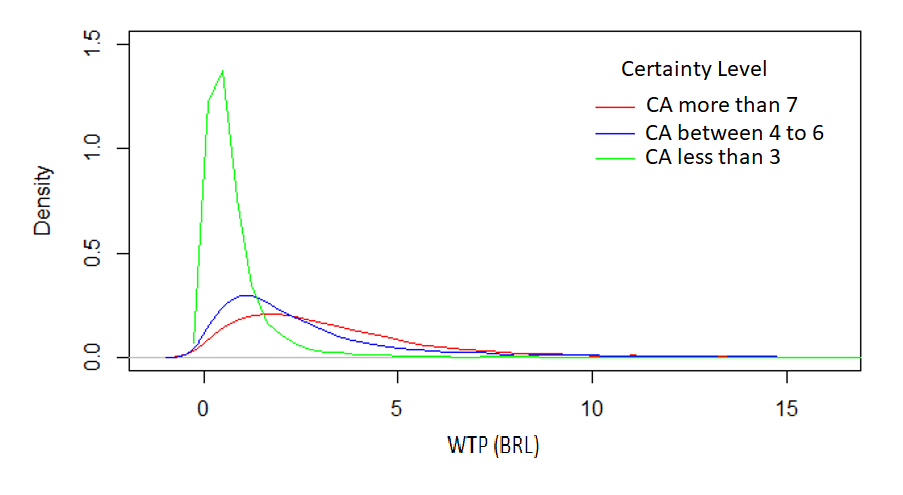
\includegraphics{dist_WTP_CArisk.png}
\caption{WTP distribution of risk of death reduction by CA.}
\end{figure}

\begin{figure}
\centering
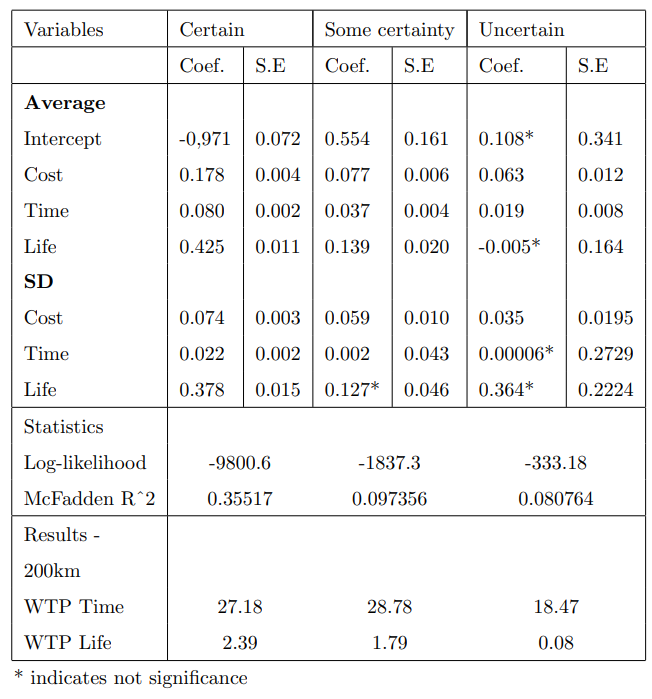
\includegraphics{table17.png}
\caption{.}
\end{figure}

\hypertarget{expanded-model}{%
\subsection{EXPANDED MODEL}\label{expanded-model}}

The expanded model was estimated to observe the systematic heterogeneity
of preferences, which can occur due to different socioeconomic
characteristics or to different travel behaviour from each respondent.
Thus, we added the following characteristics to the general model:

\begin{verbatim}
1. Household Income
2. Number of children
3. Trip Purpose
4. Traffic accident question`s position in questionnaire
5. Occurrence of traffic accident in last 5 years
6. Gender
7. Age group
8. If committed any traffic infractions
9. If the respondent imagined himself as being alone or with company.
\end{verbatim}

From the items listed above, numbers 2, 3 and 5 did not present
statistical significance at the level of 90\%, that is, they do not
influence the respondents` preferences when making a choice between
routes A and B, as shown in Table. All other characteristics were
significant at 99\%, except for the position of the accident question,
which was significant at 95\%.

\begin{figure}
\centering
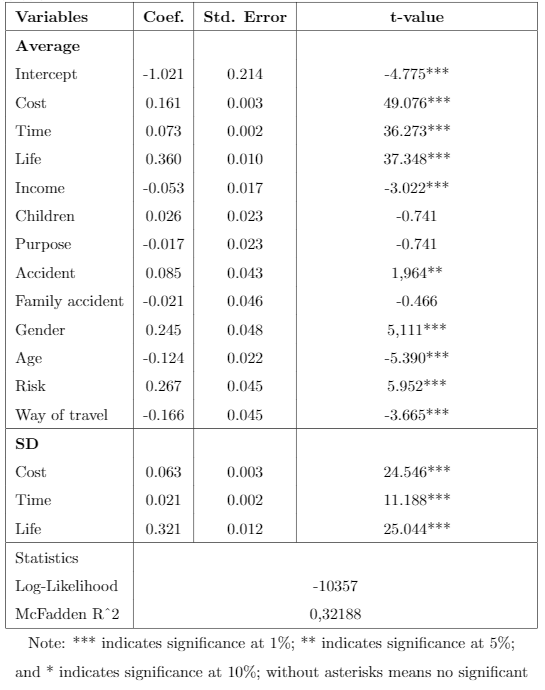
\includegraphics{table16.png}
\caption{Mixed Logit Model Result controled by socioeconomic
characteristics and travel behavior.}
\end{figure}

Table shows the WTP values calculated for each characteristic with
significance equal to or higher than 95\%. Female respondents declared
to be willing to pay considerably more for safety than male subjects, in
contrast to the WTP for time savings, which was more valued by the male
respondents, except with a smaller disparity.

\begin{figure}
\centering
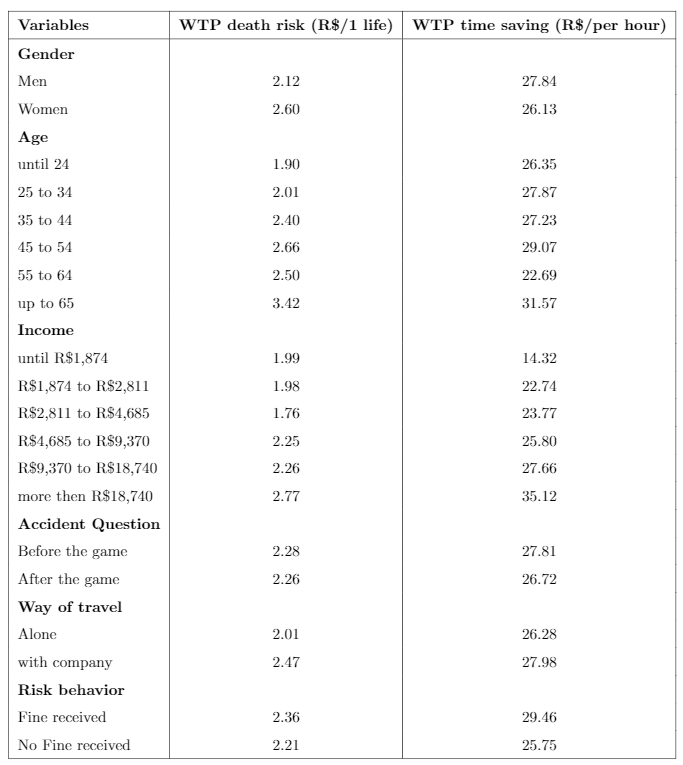
\includegraphics{WTPsocio.png}
\caption{WTP by socioeconomic characteristics.}
\end{figure}

For safety as for time savings, the age group and income group are
proportional to he willingness to pay, as expected. That is, the older
and the better financial conditions, the higher the willingness to pay.
It is also higher when the respondent imagined himself traveling
accompanied. In this case, the subject probably considered dividing the
toll cost between driver and passengers or considered that the benefits
are multiplied by the number of occupants in the car.

The respondents who received a fine for any kind of traffic infraction
in the last 12 months were classified as having risky behaviour, also
known as Risk Lovers. As expected, they are willing to pay higher prices
to reduce travel time and to reduce risk than respondents who didn't
present such behaviour.

\hypertarget{references}{%
\section*{References}\label{references}}
\addcontentsline{toc}{section}{References}

\hypertarget{refs}{}
\leavevmode\hypertarget{ref-beck2016can}{}%
Beck, M.J., Fifer, S., Rose, J.M., 2016. Can you ever be certain?
Reducing hypothetical bias in stated choice experiments via respondent
reported choice certainty. Transportation Research Part B:
Methodological 89, 149--167.

\leavevmode\hypertarget{ref-hensher2003mixed}{}%
Hensher, D.A., Greene, W.H., 2003. The mixed logit model: The state of
practice. Transportation 30, 133--176.

\leavevmode\hypertarget{ref-hess2005estimation}{}%
Hess, S., Bierlaire, M., Polak, J.W., 2005. Estimation of value of
travel-time savings using mixed logit models. Transportation Research
Part A: Policy and Practice 39, 221--236.

\leavevmode\hypertarget{ref-pompermayer2017simulaccao}{}%
Pompermayer, F.M., 2017. Simulação de parceria público-privada para as
rodovias federais: Impactos sobre orçamento fiscal, usuários e
contribuintes. Instituto de Pesquisa Econômica Aplicada (Ipea).

\leavevmode\hypertarget{ref-sen1993internal}{}%
Sen, A., 1993. Internal consistency of choice. Econometrica: Journal of
the Econometric Society 495--521.

\leavevmode\hypertarget{ref-train2002discrete}{}%
Train, K.E., 2002. Discrete choice methods with simulation. Cambridge
university press.


\end{document}


